\documentclass[10pt]{beamer}%
 \usetheme[progressbar = foot, background=light, numbering=none]{metropolis} 
 %\usecolortheme[]{owl} %owl-defined colours will be available as OwlRed, OwlGreen, and so forth.
 %\setbeamercolor{title separator}{fg=OwlGreen}
%\setsansfont{Ubuntu}
%\setmonofont{Ubuntu Mono}
% % input
% 
\useoutertheme{split}
%\setbeamertemplate{footline}{\small \insertauthor}

\usepackage[utf8]{inputenc}%
 \usepackage{lmodern} %Type1-font for non-english texts and characters
 \usepackage[USenglish]{babel} %francais, polish, spanish, ...
 \usepackage[T1]{fontenc}
% 
 \usepackage{ragged2e}%for text justification by default
 \justifying
% 
 % graphics
 %% Figures %%%%%%%%%%%%%%%%%%%%%%%%%%%%%%%%%%%%%%%%%%%%%%%%%%
 \usepackage{graphicx}
 
 \hypersetup{pdfstartview={Fit}} % fits the presentation to the window when first displayed
 
 \title[Software workshop]{Software workshop}
 \subtitle{Which software will make my PhD (slightly) easier?}
 \date{\today}
 \author[EE PhD retreat 2019]{Timoth\'ee Bonnet, based on slides from \textbf{Jessica} and \textbf{Christiana}}

%%%%%%%%%%%%%%%%%%%%%%%%%%%%%%%%%%%%%%%%%%%%%%
\begin{document}

\begin{frame}
\maketitle
\end{frame}
%%%%%%%

\begin{frame}{}
    \begin{itemize}
    \item Keeping track of the literature
    \item Reference management
    \item Reports, manuscripts, presentations, notes \dots
    \item Data analysis
    \item Data Management
        \end{itemize}

\end{frame}
%%%%%%%%%

\begin{frame}{Keeping track of the literature: Google scholar}

    \begin{itemize}
   \item Quick, broad but non-repeatable Search engine
   \item Keep track of your citations (more than on Web of Science !!)
   \item Get updates based on your citations
   \item Follow people in your field
   \item Create alerts for specific keywords
 \end{itemize}

\end{frame}
%%%%%%%%

\begin{frame}{Keeping track of the literature: Web of Science and Scopus}

    \begin{itemize}
   \item Slow, targeted and repeatable search engine (recommended for literature review)
    \item Keep track of your citations (ResearcherID)
    \item Create alerts for specific keywords
 \end{itemize}

\end{frame}
%%%%%%%


\begin{frame}{Keeping track of the literature: Social media}
twitter et al
\end{frame}
%%%%%%%


\begin{frame}{Keeping track of the literature: Journal email alerts}
\end{frame}
%%%%%%%


\begin{frame}{Reference management}


\includegraphics[width=0.4\textwidth]{Figures/readcube} \hfill

\includegraphics[width=0.2\textwidth]{Figures/papers}


\includegraphics[width=0.25\textwidth]{Figures/reftruc}\hfill

\includegraphics[width=0.25\textwidth]{Figures/endnote}\hfill

\includegraphics[width=0.25\textwidth]{Figures/citavi}


\includegraphics[width=0.3\textwidth]{Figures/zotero}\hfill 

\includegraphics[width=0.3\textwidth]{Figures/mendeley}

\end{frame}
%%%%%%%
\begin{frame}{Reference management}

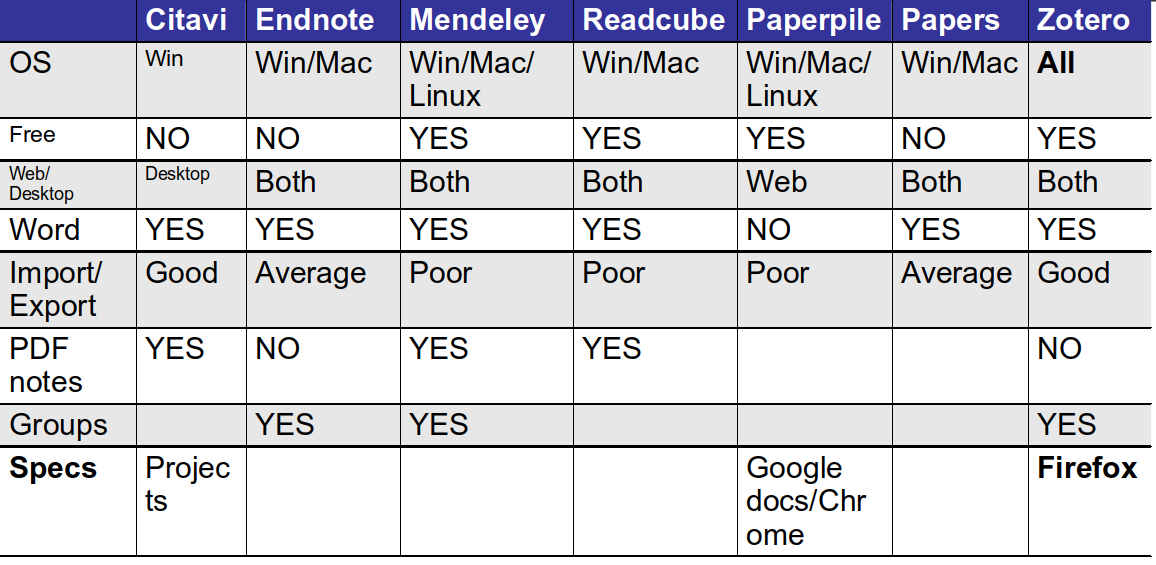
\includegraphics[width=\textwidth]{Figures/comp}

\end{frame}
%%%%%%%

\begin{frame}{Reports, manuscripts, presentations, notes \dots}
 
\end{frame}
%%%%%%%%


\begin{frame}{Reports, manuscripts, presentations, notes \dots}
\centering
\textbf{Mind mapping}
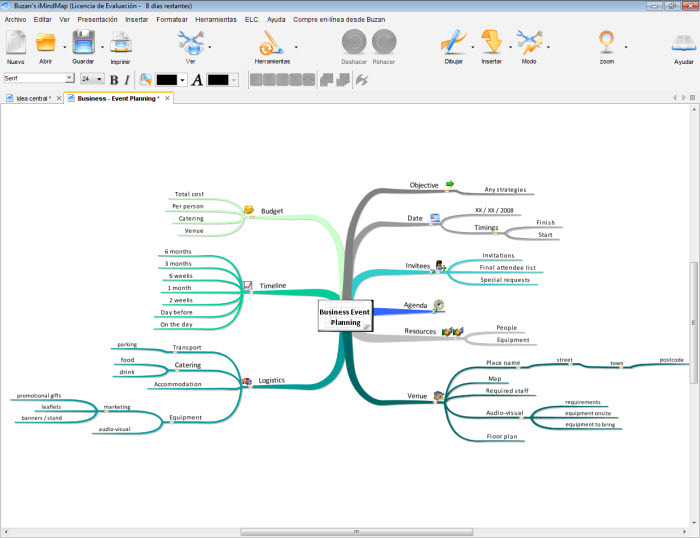
\includegraphics[width=0.9\textwidth]{Figures/mindmaps}
\end{frame}
%%%%%%%%

\begin{frame}{Data analysis, statistics\dots }
\begin{center}

\includegraphics[width=0.8\textwidth]{Figures/ralert}
\end{center}
\begin{itemize}
 \item Free to use
\item Large community
\item Highly versatile
\end{itemize}
\end{frame}
%%%%%%%

\begin{frame}{Data analysis, statistics\dots }

\includegraphics[width=0.2\textwidth]{Figures/rsname}
\vspace{-0.5cm}

\centering
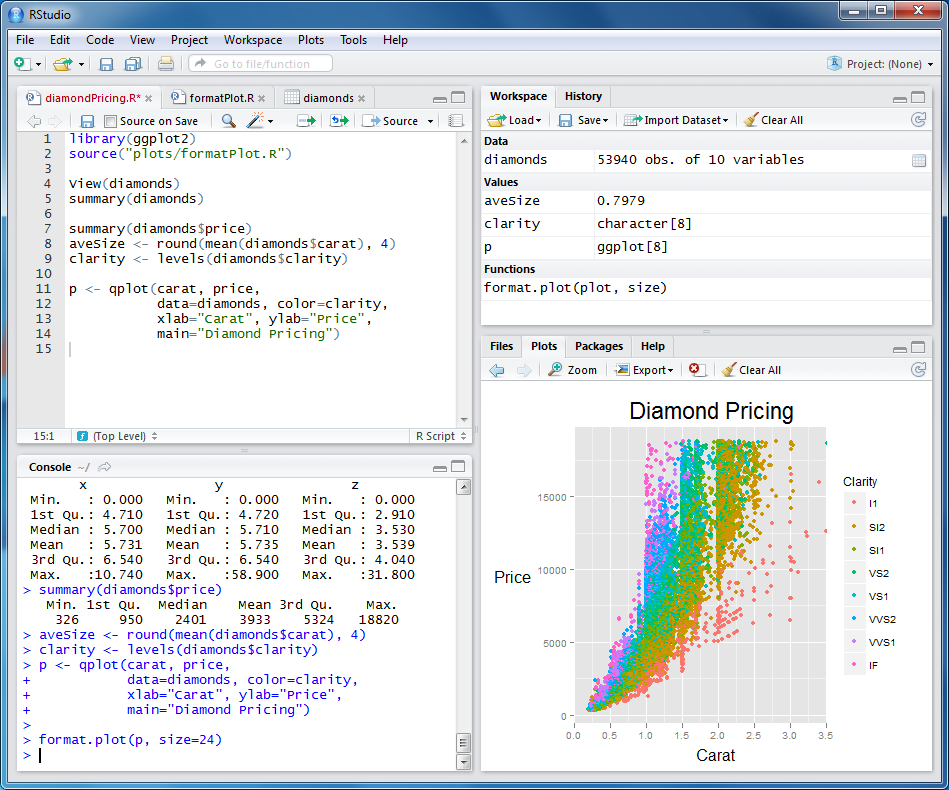
\includegraphics[width=0.7\textwidth]{Figures/Rstudio2}
\end{frame}
%%%%%%%

\begin{frame}{Data analysis, statistics\dots }
    \begin{block}{Find help:}
        \begin{itemize}
         \item The Internet
         \item Colleagues
         \item (books: learn BEFORE you have an issue)
         \item Courses, workshops, consulting
        \end{itemize}
    
    
\includegraphics[width=\textwidth]{Figures/bdsi}
    BDSI: Terry Neeman, Marcin Adamski, Cameron Jack, myself \dots
    \end{block}

\end{frame}
%%%%%%%

\begin{frame}{Data management}
\alert{Regular back-ups} \hfill \alert{Multiple locations/types}

\begin{itemize}
 \item  RSB personal folder (50GB)
    \item Personal Hard Disk (not where your computer is)
\item Alternative cloud storage
\end{itemize}

\end{frame}
%%%%%%%


\begin{frame}{Data management: repositories}
\end{frame}
%%%%%%%

\begin{frame}{Data management: Version controls / Github}
\end{frame}
%%%%%%%

\end{document}
